\section{Data Analysis}
With the data I collected, a total of 56 participants were involved in my research study - giving me a total of 560 results to analyse (280 per stage). This data collected was then split into two separate CSV files each holding the appropriate data regarding each stage. The data was used in a series of Z-Tests in R (See \hyperref[append:g]{\italic{Appendix G}}) and appropriate charts were generated to visualise the data in each stage (See Fig~\ref{stage-1-graph} and Fig~\ref{stage-2-graph}).
Due to the large sample size from the data, the Binomial distribution is approximated with the population mean \(\mu = np\) (where \italic{n} is the total sample size and \italic{p} is the probability) and standard deviation \(\sigma = \sqrt{np(1-p)}\).
\\
With this, the Z-Test is calculated like so (where \italic{$x$} is the amount of successful trials in the Binomial Test) \cite[Chapter~6]{zar-jerrold}
\[z = \frac{(x - \mu ) }{\sigma }\]

\subsection{Hypothesis Results}
\subsubsection{Hypothesis 1}
\italic{When unaware, the Artefact (M-A System) is picked more often than Human designed interiors by participants}.\\
In this stage participants were required to select, out of each pair, which room they preferred - to test this hypothesis an upper-tailed Z-Test was used.
This test was used to check to see if the Artefact interiors were selected significantly more than human designs. The Z-Test returned a value of 0.84, when calculating the P value it returns as 0.2005. With this we have failed to reject the null hypothesis - as the value is not statistically significant enough at P $<$ 0.05.
\\
\subsubsection{Hypothesis 2}
\italic{When notified, the participant is not able to distinguish
between Human and Artefact (M-A System) interiors}.\\
In this stage, participants were notified of the Artefact and were told to select, out of the same 5 pairs they saw in Stage 1, which room they believe was made by the Artefact. By completing another upper-tailed Z-Test to check if human designs were selected more than the Artefacts, we return a Z score of -1.67 and can calculate a P value of 0.9525. With this, we have again failed to reject the null hypothesis as it is not significant enough at P $<$ 0.05.

\begin{figure}[!ht]
    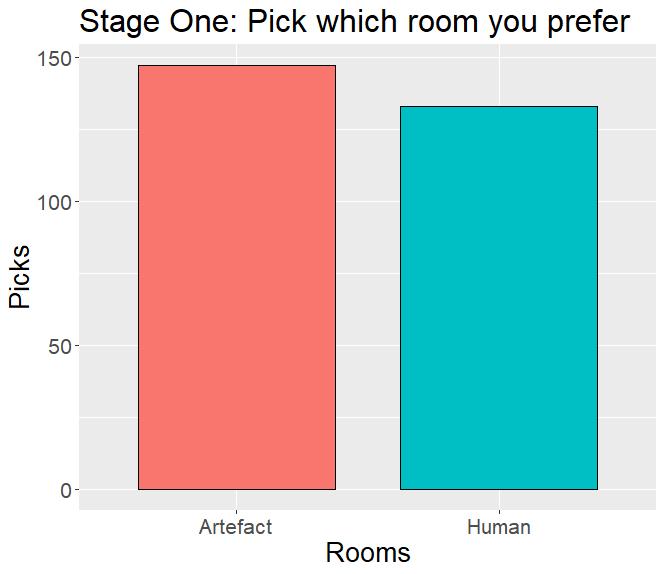
\includegraphics[width=\columnwidth]{./Images/stage-1-picks-graph.png}
    \centering
    \caption{Bar chart representing the data from Stage 1}
    \label{stage-1-graph}
\end{figure}

\begin{figure}[!ht]
    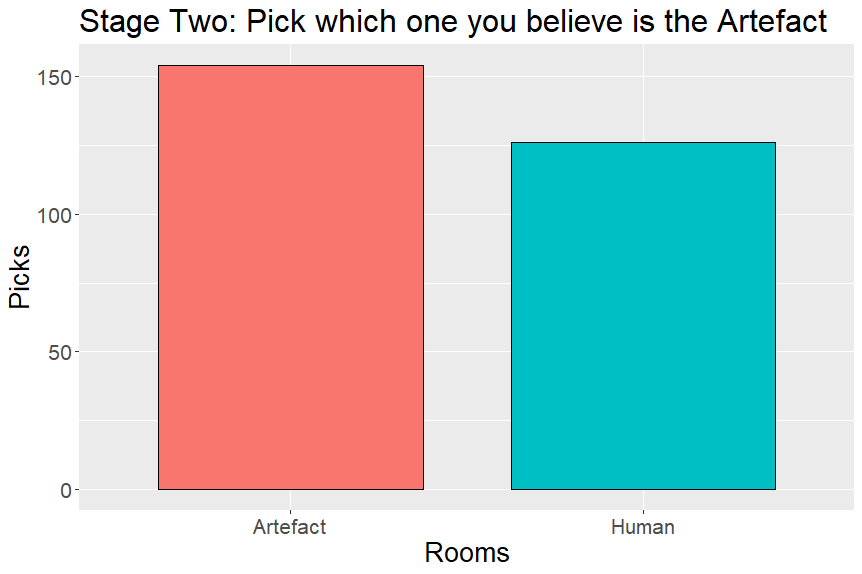
\includegraphics[width=\columnwidth]{./Images/stage-2-picks-graph.png}
    \centering
    \caption{Bar chart representing the data from Stage 2}
    \label{stage-2-graph}
\end{figure}